\section{Ejercicio 3}
\label{ej3}
\subsection{Introducción}

\paragraph{}
Para la resolución de este ejercicio se debía desarrollar e implementar una heurística constructiva  para resolver el problema de encontrar un \mc dado un grafo simple.


\subsection{Explicación}

\paragraph{}
En una primera aproximación al problema, se pensó un algoritmo bastante sencillo. La idea del mismo radicaba en ir tomando los nodos en orden de grados, es decir, comenzando con los de mayor grado hasta llegar a los de menor grado. De esta forma, uno puede pensar que al tomar primero los vértices de mayor grado, hay mas chances de encontrar una clique de mayor tamaño.

\paragraph{}
Esto es claramente una heurística válida que utiliza la técnica de algoritmo goloso. Pero es claro también que se pueden encontrar fácilmente ejemplos de grafos en los que dicho algoritmo funcione tan mal como uno quiera.

\paragraph{}
A fines de evitar en cierto grado muchos casos para los cuales este algoritmo funciona mal, se planteó uno nuevo que utiliza la misma idea pero que la misma no se realiza sobre todos los nodos del grafo sino que se hace sobre un subconjunto de los mismos. Para formar dicho conjunto, se implementó un algoritmo que revisa todas las combinaciones de 2 vértices distintos (siempre y cuándo haya 2 o más vertices en el grafo) que sean vecinos entre sí y se guarda en un conjunto de vértices aquellos que sean vecinos a ambos vértices y además se guardan los 2 vértices en cuestión. Esto se repite para cada posible combinación de vértices de a 2, guardando siempre el conjunto más grande que se haya encontrado completado de la forma antes mencionada.

\paragraph{}
Una vez encontrado este subgrafo, se procede a realizar el algoritmo goloso antes mencionado pero sobre dicho subgrafo, es decir, se busca el nodo con mayor grado en ese subgrafo y se coloca en un conjunto, el cuál será devuelto como clique al terminar el algoritmo. Luego, para el resto de los nodos del subgrafo, se va tomando de a uno a la vez en orden de mayor a menor grado (considerando sólo los adyacentes que pertenecen al subgrafo) y se verifica que sea adyacente a todos los que pertenecen a la clique. Si lo es, entonces se lo inserta en el conjunto sino se lo descarta. Finalmente, se prosigue con estos pasos hasta haber intentado con todos los nodos del subgrafo devolviendo entonces la clique encontrada.

\paragraph{}
A continuación se adjunta el pseudocódigo del algoritmo constructivo antes descripto y el de las funciones auxiliares pertinentes. En los mismos, utilizaremos a ``n'' como forma de expresar la cantidad de nodos pertenecientes al grafo.

\vspace{2em}
\incmargin{3em}
\linesnumbered
\restylealgo{boxed}
\footnotesize 
\textbf{cliqueConstructivo}(G: grafo) \\
\begin{algorithm}[H]
	\BlankLine
	frontera = mayorFronteraEnComun(G) \tcp*{\Ode{n^3}}
	res = $\emptyset$\tcp*{\Ode{1}}
	\BlankLine

	\textbf{mientras} frontera $\neq\ \emptyset$\\

		\tab v = elMasRelacionado(G,frontera)\tcp*{\Ode{n^2}}
		\tab \textbf{si} esVecinoDeTodos(G,res,v)\tcp*{\Ode{n}}
			\tab \tab \textbf{insertar} v \textbf{en} res\tcp*{\Ode{log(n)}}
		\tab \textbf{fin si}\\
		\tab \textbf{eliminar} v \textbf{de} frontera\tcp*{\Ode{log(n)}}
	\textbf{fin mientras}\\

	\textbf{si} res $==\ \emptyset$\tcp*{\Ode{1}}
		\tab \textbf{insertar} $v_0$ \textbf{en} res\tcp*{\Ode{1}}
	\textbf{fin si}\\

	\textbf{devolver} res
\caption{Pseudocódigo del algoritmo constructivo}
\end{algorithm}

\vspace{3em}

\textbf{mayorFronteraEnComun}(G: grafo) \\
\begin{algorithm}[H]
	\BlankLine
	aux = $\emptyset$\tcp*{\Ode{1}}
	res = $\emptyset$\tcp*{\Ode{1}}
	\textbf{paratodo} u,v $\in\ V_{G}$ \textbf{tq} (u,v) $\in\ X_{G}$ \\
		\tab aux = (adyacentes(G,u) $\cap$ adyacentes(G,v)) $\cup$ u $\cup$ v\tcp*{\Ode{n}}
		\tab \textbf{si} \#aux $>$ \#res\tcp*{\Ode{1}}
			\tab \tab res = aux\tcp*{\Ode{1}}
		\tab \textbf{fin si}\\
	\textbf{fin paratodo}\\

	\textbf{devolver} res

\caption{Pseudocódigo de un algoritmo secundario al constructivo}
\end{algorithm}
 
\normalsize

\paragraph{}
El pseudocódigo de las funciones \textit{elMasRelacionado, esVecinoDeTodos} y \textit{adyacentes} no se detalla ya que no son algoritmos de gran complejidad. Igualmente, se explicarán brevemente a continuación.\\
En el caso de \textit{elMasRelacionado}, recibe dos parámetros, un grafo y un conjunto de vértices. Esta función devuelve el vértice de mayor grado del grafo inducido por los vértices de ese conjunto. La función \textit{esVecinoDeTodos} recibe un grafo, un vértice y un conjunto de vértices. Devuelve verdadero si y sólo si el vértice es adyacente a todos los vértices del conjunto. Por último, en el caso de la función \textit{adyacentes}, recibe un grafo y un vértice como parámetros y devuelve el conjunto de todos los vértices adyacentes al pasado como parámetro.


\subsection{Análisis de la complejidad del algoritmo}
\label{complejidad3}
\paragraph{}
Para realizar el siguiente análisis de complejidad vamos a remitirnos al pseudocódigo de la función \textit{AlgoritmoConstructivo} adjunto en la sección anterior. Cabe recordar que cada vez que se haga mención a ``n'' nos estaremos refiriendo a la cantidad de nodos del grafo al que se quiere analizar.\\
En la primer línea se realiza una llamada a la función \textit{mayorFronteraEnComun} y una asignación. Estas 2 operaciones tienen una complejidad de \Ode{n^3}. Más adelante se explicará el por qué de la misma. Luego, dentro del ciclo, la función que mayor complejidad temporal tiene es \textit{elMasRelacionado} y la misma es \Ode{n^2}. Esta complejidad se debe a que para cada vértice del grafo inducido por el conjunto de vértices pasado como parámetro, se debe calcular cuántos vecinos tiene dentro de ese grafo, para lo que se debe recorrer todo el conjunto una vez por cada vértice. Como a lo sumo puede haber ``n'' vértices en ese conjunto, debo recorrerlo ``n'' veces por cada vértice. Entonces, su complejidad es \Ode{n^2}.\\
Deberiamos ver ahora cuántas veces va a ejecutarse el ciclo. Este finalizará una vez que el conjunto llamado ``frontera'' quede vacío. Este arranca con el valor de la mayor frontera en común, por lo que a lo sumo puede ser de tamaño ``n'', es decir, todos los vértices pueden pertenecer a él en el peor caso. Podemos observar además, que en cada paso del ciclo, su tamaño disminuye en uno (línea 8, al eliminar un vértice del conjunto) , por lo que a lo sumo el ciclo se ejecutará ``n'' veces. Como la función más compleja dentro del ciclo era \textit{elMasRelacionado} con una complejidad de \Ode{n^2} y la misma se ejecutará ``n'' veces, entonces la complejidad total temporal del ciclo es de \Ode{n^3}. Por lo tanto, la complejidad del algoritmo constructivo es de \Ode{n^3}.

\paragraph{}
Para completar este análisis, falta justificar por qué la función \textit{mayorFronteraEnComun} tiene complejidad \Ode{n^3}.\\
En el caso de la intersección, sólo hace falta recorrer una sola vez la lista de todos los vértices para saber cuáles son vecinos a ambos nodos a la vez, y la unión de dicha intersección con los vértices ``u'' y ``v'' tiene complejidad logarítmica, por lo que dicha instrucción tiene complejidad \Ode{n}. Pero esta sentencia se ejecuta tantas veces como se ejecute el ciclo \textit{for}, así que para saber la complejidad total, debemos conocer las veces que se ejecuta el ciclo: éste se ejecuta tantas veces como aristas haya. En el peor caso, si hay ``n'' nodos entonces puede haber hasta ``$n^2$'' aristas. Por lo que el ciclo se ejecutará a lo sumo $n^2$ veces\footnote{La complejidad podría verse como \Ode{m} pero como se eligió una matriz de adyacencia para modelar el grafo, para recorrer todas las aristas es necesario pasar por cada valor de la matriz de adyacencia, por eso es que se toma como complejidad \Ode{n^2} y no \Ode{m}}. Finalmente, la complejidad total de \textit{mayorFronteraEnComun} es \Ode{n^3}. 


\subsection{Resultados}

\paragraph{}
A continuación se presentan los gráficos provenientes de las pruebas realizadas con archivos generados al azar. La forma en la que fueron generados estos archivos de entrada es explicada en la sección [\ref{anexo}].


%primeras 2 imagenes
\begin{figure}[htb]
    \begin{minipage}{\textwidth}
	\begin{center}
		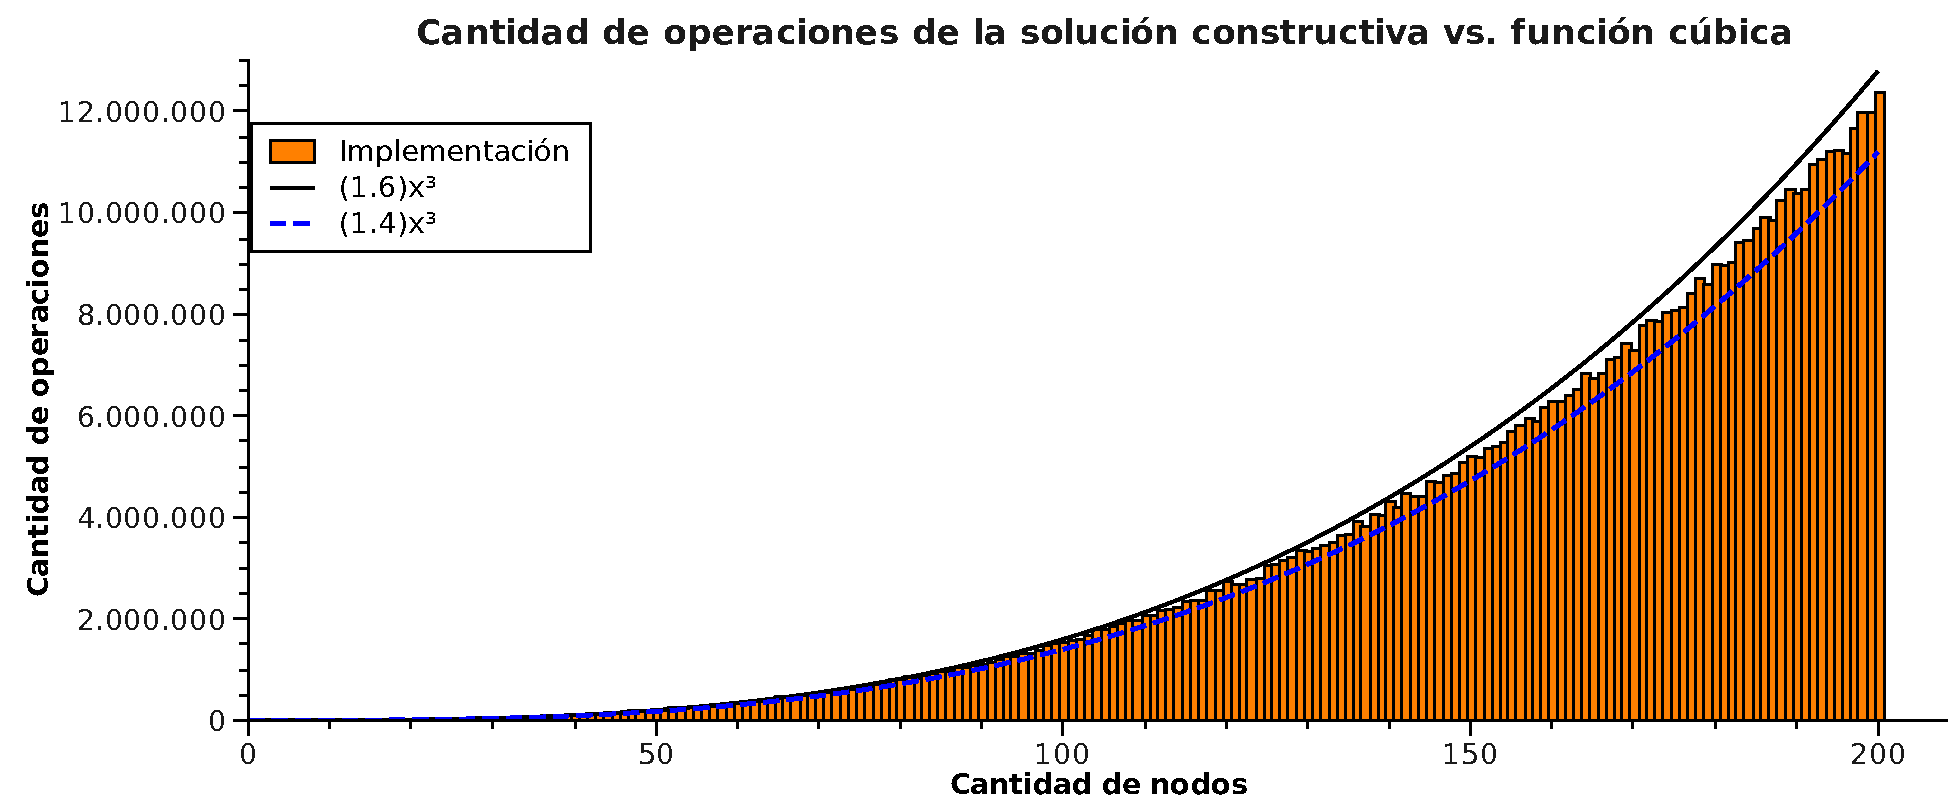
\includegraphics[width=\textwidth]{./otros/graficos/operaciones_200nodos1_ej3.pdf}
		\caption{Muestra el comportamiento del algoritmo constructivo, comparando cantidad de nodos contra cantidad de operaciones. La probabilidad de aparición de ejes en esta muestra fue del 50\%}
		\label{ej3contarOp}
	\end{center}
    \end{minipage}

\vspace*{3cm}

    \begin{minipage}{\textwidth}
	\begin{center}
		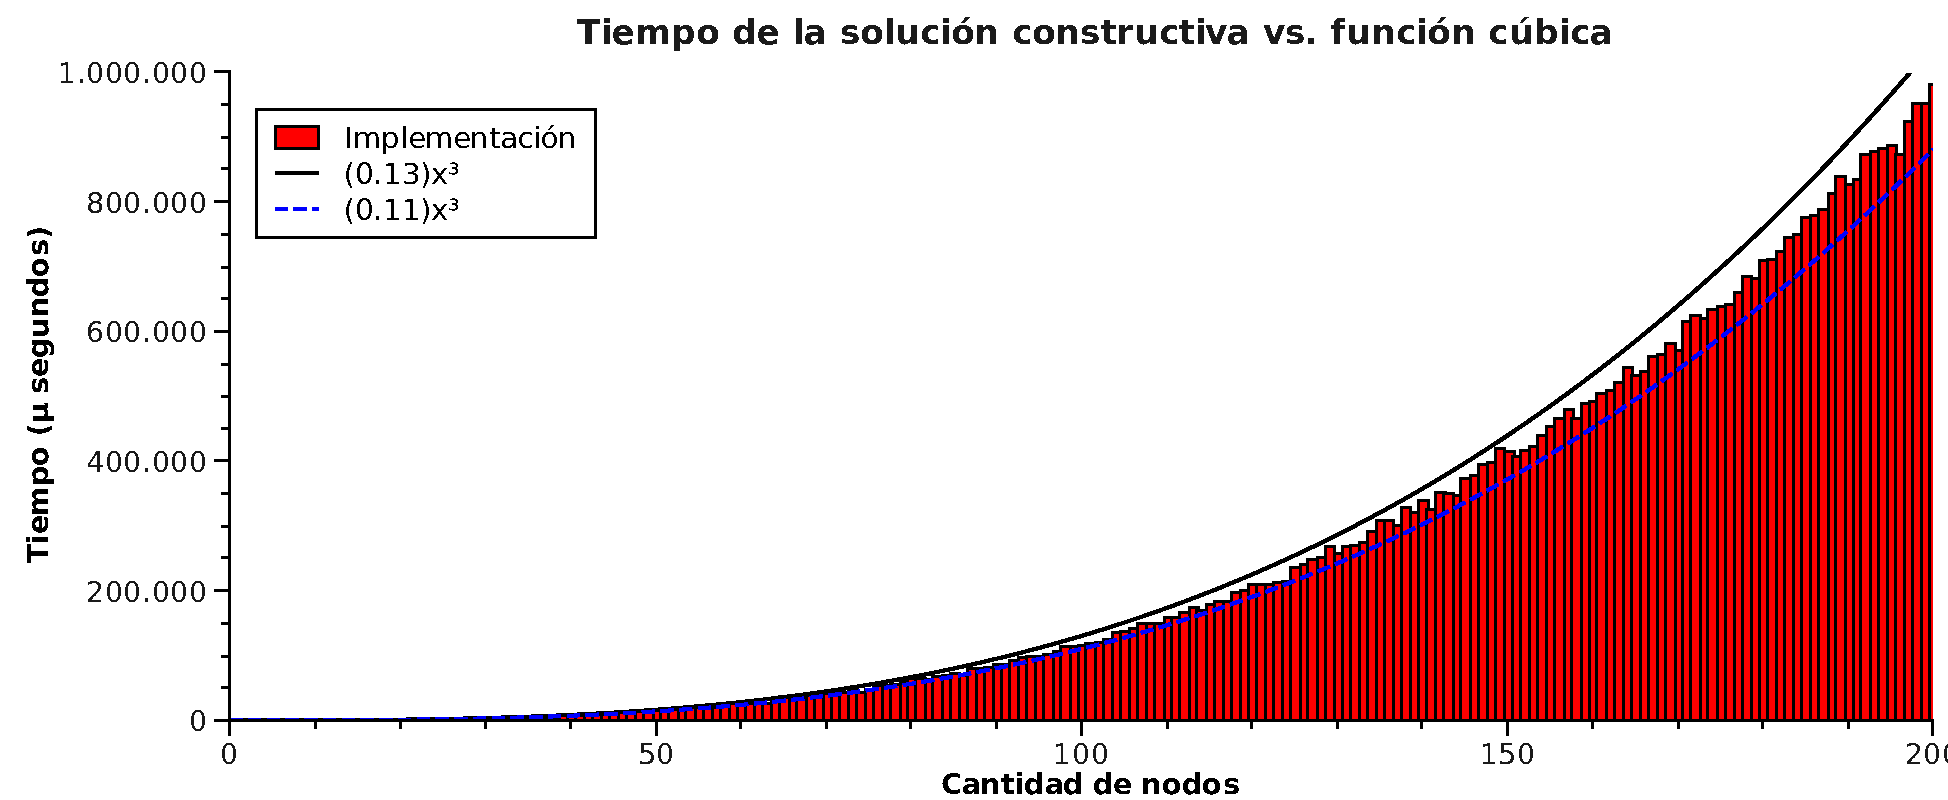
\includegraphics[width=\textwidth]{./otros/graficos/tiempo_200nodos1_ej3.pdf}
		\caption{Muestra el comportamiento del algoritmo constructivo, comparando cantidad de nodos contra el tiempo medido en microsegundos. La probabilidad de aparición de ejes en esta muestra fue del 50\%}
		\label{ej3contarTiempo2}
	\end{center}
    \end{minipage}

\end{figure}


\subsection{Debate y conclusiones}
\paragraph{}
Si observamos los gráficos adjuntos en la sección anterior, podemos decir que para estos casos de pruebas el algoritmo constructivo pareciera haberse comportado como se esperaba. En ambos casos, los datos arrojados luego de realizar pruebas con el algoritmo pueden ser acotados tanto por debajo como por arriba por una función cúbica.

\paragraph{}
Para este análisis se realizaron varias pruebas, en las que se hizo variar tanto la cantidad de nodos pertenecientes a los grafos, como así también la cantidad de ejes. En todas ellas, pudo notarse una gran similitud en los datos arrojados, es decir, todas se comportaban como se esperaba y podían ser acotadas por arriba y por abajo por una función cúbica.\\
La única diferencia notable entre distintas pruebas fue que en los casos de prueba en los que había más ejes, es decir, en aquellos casos en que los grafos eran más densos, la constante que acompañaba a la función cúbica era un poco mayor. A pesar que esta diferencia existía, no era muy notable como para incluir gráficos que la mostraran.

\paragraph{}
Podemos concluir entonces que el análisis realizado en la sección [\ref{complejidad3}] era correcto y que la complejidad de este algoritmo es de orden cúbico.
